\appendixsection{Исследование квантового преимущества}

В этой части мы численно исследуем преимущество квантового оптимизатора по
сравнению с алгоритмом Бабаи. Рассматриваемый критерий измерения — это качество
коротких векторов для задачи ближайшего вектора (CVP). Качество короткого
вектора положительно коррелирует с эффективностью получения гладких
соотношённых пар в более эффективном методе факторизации Шнорра. Поскольку в
настоящее время оценка аналитической сложности алгоритма QAOA остаётся открытым
вопросом, в данном обсуждении предполагается, что процедура QAOA способна
находить оптимальное решение задачи оптимизации за ограниченное время. Здесь мы
используем параметр относительного расстояния $r$ для измерения длины вектора
вместо евклидовой нормы или квадратной нормы. Параметр определяется следующим
образом:

\begin{equation}
r = \frac{\lVert \mathbf{b} - \mathbf{t} \rVert^2}{\det(\mathbf{B}'_{n,c})^{\frac{2}{n}}},
\end{equation}

\noindent где $B'_{n,c} = [B_{n,c},\, N c]$. Этот параметр использует $2/n$‑степень
определителя расширенной решётки $B'_{n,c}$ для измерения относительной длины
короткого вектора $b - t$, что позволяет в определённой степени уменьшить
влияние различий в определителе решёток на качество коротких векторов.

\subsection*{Результаты на случайных выборках}

Сначала мы исследуем производительность квантового оптимизатора и классического
алгоритма Бабаи на случайных выборках задачи CVP. Здесь мы генерируем 50
случайных примеров CVP (решётка и целевой вектор) при условиях размерности
решётки $n = 7$, точности $c = 10$ и $n = 10$, $c = 7$ соответственно. Для
каждой случайной выборки определитель решётки и целевой вектор остаются
одинаковыми — меняются только элементы главной диагонали решётки, которые
случайным образом переставляются. Результаты представлены на рис.
\ref{fig:fig08}. По горизонтальной оси отложены случайные выборки, по
вертикальной — относительное качество $r$ результирующего вектора. Синие
(жёлтые) столбцы представляют результаты классического алгоритма Бабаи
(квантовой оптимизации). Как видно на графике, результаты, полученные с помощью
квантовой оптимизации, не хуже классических, а во многих случаях существенно
лучше, то есть получены более короткие векторы.

\begin{figure}
    \centering
    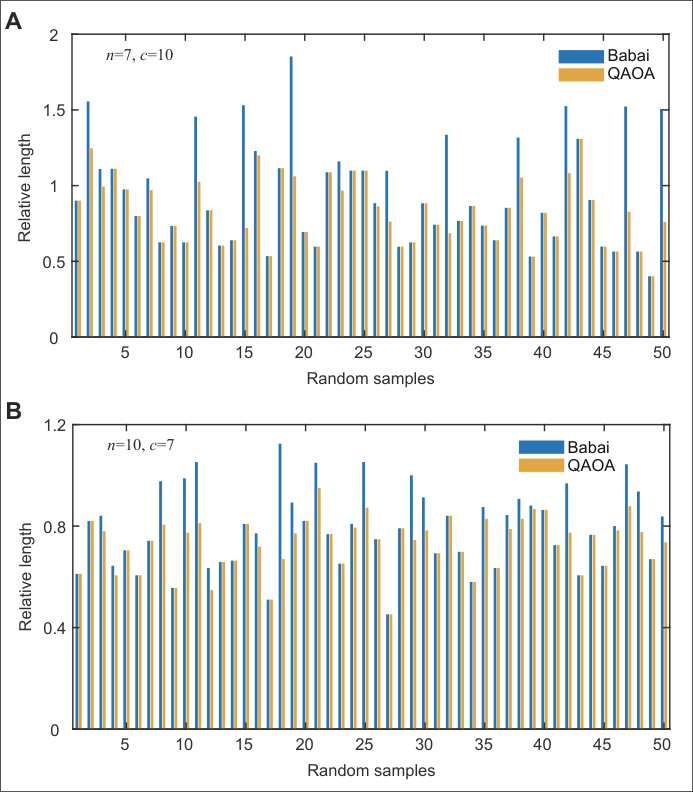
\includegraphics[scale=0.6]{inc/fig_08.png}
    \caption{
    Производительность на случайных выборках для квантового оптимизатора (QAOA)
    по сравнению с алгоритмом Бабаи. A (B) — результаты для 50 случайных
    примеров задачи CVP при условиях $n = 7$, $c = 10$ ($n = 10$, $c = 7$).
    Жёлтые (синие) столбцы представляют результаты квантового оптимизатора
    (классического алгоритма Бабаи). Можно наблюдать, что в ряде случаев
    результаты квантовой оптимизации превосходят классические.
    }
    \label{fig:fig08}
\end{figure}

\subsection*{Квантовое преимущество и точность решётки}

Мы дополнительно исследуем преимущество квантового оптимизатора при увеличении
параметра точности $c$ решётки. На рис. \ref{fig:fig09}A представлены численные
результаты при увеличении параметра $c$ от 5 до 14 для размерностей решётки $n
= 12$ и $n = 14$ соответственно. Результаты усреднены по 40 случайно
сгенерированным примерам задачи CVP для каждого набора параметров $\{n, c\}$.
Символы в виде кружков (треугольников) соответствуют результатам при $n = 12$
($n = 14$). Сплошные (пустые) символы обозначают результаты квантового
(классического) алгоритма. Погрешности отображают доверительный интервал при
стандартном отклонении, равном единице.

В обоих случаях, при $n = 12$ и $n = 14$, после квантовой оптимизации
получаются более короткие векторы. Рассматривая случай $n = 14$ в качестве
примера, можно увидеть, что разрыв в качестве между результатами алгоритма
Бабаи и квантового алгоритма постепенно увеличивается с ростом параметра $c$.
Это указывает на то, что качество вектора после квантовой оптимизации в среднем
выше, чем у алгоритма Бабаи, при увеличении определителя решётки.

Кроме того, на рис. \ref{fig:fig09}B приведена доля выборок, где квантовая
оптимизация дала преимущество, относительно всех 40 случайных примеров. Эти
доли показаны синими и оранжевыми столбцами для случаев $n = 12$ и $n = 14$
соответственно. Мы обнаружили, что для $n = 12$ доля квантового преимущества
составляет примерно 0{,}5, а для $n = 14$ она увеличивается до 0{,}65.
Результаты свидетельствуют о том, что квантовое преимущество становится более
заметным при увеличении размерности решётки. Эти результаты будут дополнительно
подтверждены в следующем разделе.

\subsection*{Квантовое преимущество и размерность решётки}

Здесь мы исследуем зависимость преимущества квантового оптимизатора от
размерности решётки до $n = 14$. Для каждой размерности $n$ результаты
усреднены по 40 случайным выборкам при $c = n$. Как показано на рис.
\ref{fig:fig10}A, качество вектора после квантовой оптимизации в среднем выше,
чем при использовании классического алгоритма Бабаи.
\begin{figure}
    \centering
    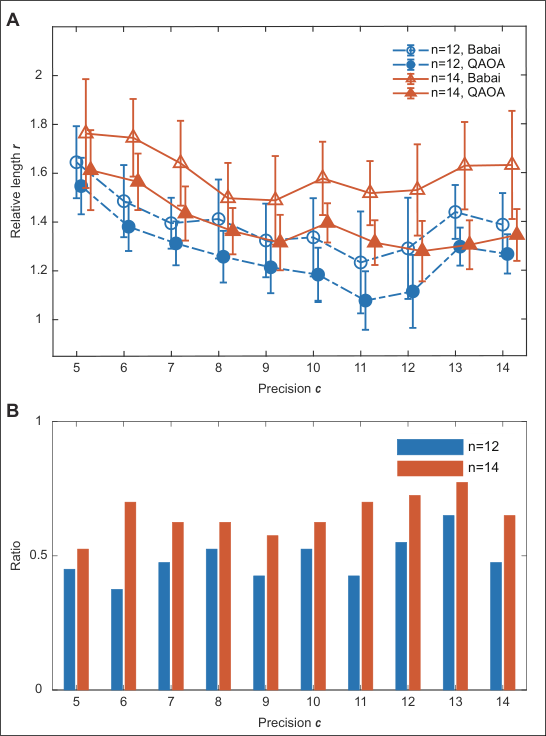
\includegraphics[scale=0.6]{inc/fig_09.png}
    \caption{
    Производительность квантового оптимизатора при увеличении точности решётки.
    A: Относительные длины для квантовых и классических методов. По
    горизонтальной оси отложен параметр точности $c$, положительно
    коррелирующий с определителем решётки. B: Доля квантового преимущества для
    40 случайных выборок, синие (оранжевые) столбцы для случая $n = 12$ ($n =
    14$). На графике видно, что в среднем квантовая оптимизация даёт лучшие
    результаты, особенно при больших значениях определителя (связанного с $c$).
    }
    \label{fig:fig09}
\end{figure}

Иначе говоря, с помощью квантовой оптимизации можно найти более короткий
вектор. Разрыв в качестве между квантовыми и классическими результатами
становится более заметным с увеличением размерности решётки, что означает, что
преимущество квантового метода возрастает в более крупных системах. Также мы
подсчитали долю квантового преимущества среди 40 случайных выборок,
представленных на рис. \ref{fig:fig10}B. Эта доля возрастает с увеличением
размерности, что согласуется с различием тенденций на графиках качества
векторов на рис. \ref{fig:fig10}A. Оба результата указывают на то, что
преимущества квантовых методов будут становиться всё более очевидными с ростом
размерности решётки.

\begin{figure}
    \centering
    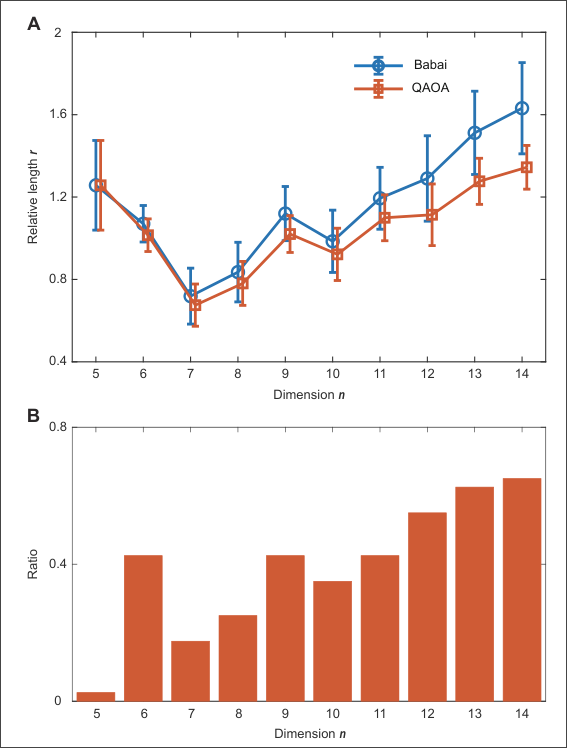
\includegraphics[scale=0.6]{inc/fig_10.png}
    \caption{
    Производительность квантового оптимизатора при увеличении размерности
    решётки. A: Относительная длина векторов для квантового и классического
    методов. По горизонтальной оси отложена размерность решётки $n$. Результаты
    усреднены по 40 случайным выборкам при $c = n$. Погрешности отображают
    доверительный интервал при стандартном отклонении, равном единице. B: Доля
    квантового преимущества среди 40 случайных выборок. Можно заметить, что
    разрыв в относительном расстоянии между квантовыми и классическими
    результатами увеличивается с ростом размерности решётки.
    }
    \label{fig:fig10}
\end{figure}
